\capitulo{5}{Aspectos relevantes del desarrollo del proyecto}

A medida que avanzaba con el proyecto han ido surgiendo algunos hitos importantes que voy a remarcar en este capítulo.

\section{IDE: Kinetis vs MCUXpresso}\label{sec:ARKinetisvsMCUX}
Como ya vimos en el apartado de herramientas se han utilizado dos \extranjerismo{IDEs}, ambos dos creados por la misma empresa, NXP. 
En un primer momento se comenzó utilizando Kinetis Design Studio puesto que mis tutores me facilitaron algunas prácticas realizadas con ese programa de cara a familiarizarme con ello. Tras la realización de las prácticas enseguida me di cuenta de que estaba bastante anticuado y que las nuevas versiones de \extranjerismo{drivers} y \extranjerismo{middelware} no funcionaban correctamente.
Es por ello que decidí migrar hacia MCUXpresso. Este cambio hizo que tuviera que volver a familiarizarme con el nuevo IDE y la manera de programar el hardware a bajo nivel con la herramienta \extranjerismo{Config Tools}. Aunque KDS estuviera anticuado, en lo referente al uso de esta herramienta era algo más sencillo. A favor de la MCUX diré que incluye decenas de programas de ejemplo con los que poder probar y comprender su funcionamiento, además de un montón de \extranjerismo{drivers} que habilitan la instalación de un gran número de sensores. También se puede observar que MCUXpresso cuida más la limpieza y simplicidad de las interfaces a la hora de interactuar con ella. Una vez comprendes como funciona la programación de periféricos, relojes y pines, lo cual no es sencillo en un principio, programar un sistema embebido se convierte en algo sencillo.

\section{FRDM K64F vs Arduino}\label{sec:ARK64FvsArduino}

Este proyecto también podría haberse desarrollado con las placas Arduino UNO, las cuales son muy parecidas en cuanto a su funcionamiento y uso de periféricos. Además, utilizar Arduino hubiera sido más sencillo debido a que los pines vienen ya configurados, al igual que los relojes y tan solo hubiera sido enchufar y programar las funciones de las tareas que quisiéramos. Arduino también cuenta con una comunidad mayor por lo que tendríamos librerías más simples y avanzadas y mayor información en Internet de cara a resolver fallos. Entonces, ¿Por qué decidí utilizar las FRDM K64F?\\
La respuesta es simple, el objetivo de la realización de este trabajo no era simplemente desarrollar una planta piloto que realizara una tarea útil. El objetivo principal no es que los motores funcionen adecuadamente, o la pantalla, o el sensor de temperatura, etc. El objetivo principal era aprender sobre el funcionamiento de los sistemas embebidos. Es por ello que se decidieron utilizar estas placas, `puesto que ofrece al usuario mayor control sobre ella por la necesidad de ser programada a bajo nivel.
Desde un principio se ha pretendido centrar los esfuerzos en comprender como se realiza la configuración de sus pines y relojes, etc. En un entorno real, se deben conocer el funcionamiento de estos sistemas a bajo nivel puesto que, cada proyecto desarrollado en el entorno laboral necesitará que el SE cumpla con unos requisitos específicos y no exceda de ellos para disminuir el coste y tamaño del sistema. En cada proyecto se desarrollan unas placas específicas para esos requisitos y es conveniente saber su funcionamiento interno para poder diseñarlas correctamente.\\
Por otro lado, en el caso del homólogo a la placa FRDM K64F, que sería el Arduino Uno, no hubieramos podido utilizar ni FreeRTOS puesto que no dispone de reloj de tiempo real, ni lwIP debido a que su potencia es menor a la de las placas K64F. Además, con Arduino tampoco hubieramos podido \extranjerismo{debuguear} puesto que no usa OpenSDA para cargar el software. 
Debido a todo esto se optó por la utilización de las placas FRDM-K64F.


\section{RTOS}\label{sec:ARRTOS}
En el caso de los sistemas operativos en tiempo real encontramos, algunas alternativas a FreeRTOS. Las características y conceptos más importantes de FreeRTOS ya los vimos en el apartado \ref{sec:RTOS}. Como alternativa a este sistema operativo encontramos: 
\begin{description}
\item \extranjerismo{Embedded Operating System} (embOS), es un sistema operativo en tiempo real, desarrollado por la empresa SEGGER Microcontroller. Está diseñado para ser utilizado como base para el desarrollo de aplicaciones integradas en tiempo real para una amplia gama de microcontroladores. El funcionamiento es prácticamente el mismo.
\item MQX es otra opción de sistema operativo en tiempo real propuesto por NXP. Es un SO que ofrece una API sencilla y una arquitectura modular que hace que este software sea escalable.
\end{description}
El motivo de haber elegido la utilización de FreeRTOS es su presencia en un mayor número de proyectos que sus competidores. Esto hace que existan comunidades en Internet, que nos brindan mayor información y soluciones para su correcta utilización. Además de que su propio manual ya nos ofrece los pasos a seguir, es realmente sencillo de utilizar, una vez has aprendido los conocimientos básicos de su funcionamiento.

\section{Metodologías Ágiles}\label{sec:ARMetodologiasAgiles}

Como alternativas a SCRUM teníamos dos metodologías ágiles muy utilizadas y quizás más sencillas de implementar:

\begin{description}
\item[Extreme Programming XP]
Esta metodología es muy utilizada en pequeñas empresas durante sus comienzos y consolidación. Se basa en centrar sus esfuerzos en la comunicación entre clientes y empleados, potenciando las relaciones personales mediante el trabajo en equipo y promoviendo la comunicación y la eliminación de tiempos muertos.
Sus principales fases son:
\begin{enumerate}
\item Diseño y planificación del proyecto con el cliente.
\item Programación por parejas dentro del equipo de forma que ambos puedan intercambiar conocimientos consiguiendo mejores resultados.
\item Realización continua de pruebas de código.
\end{enumerate}

\item[Kanban] 
La metodología Kanban se basa en el uso de un \extranjerismo{layout} con columnas, generalmente tres, en las que se muestran las tareas que quedan por hacer: 'Pendientes', las que están en curso: 'En proceso' y las que ya se terminaron: 'Terminadas'. Cada usuario o equipo tiene la posibilidad de aumentar el número de columnas según les sea de mayor utilidad. De esta manera se tiene conocimiento sobre el estado del proyecto en tiempo real, mejorando la productividad y eficiencia del desarrollo del trabajo.
Las principales ventajas de esta metodología son:
\begin{enumerate}
\item Facilidad para la planificación de tareas.
\item Mejora en el rendimiento de trabajo del equipo.
\item Visión global de un solo vistazo.
\item Los plazos de entregas son continuos.
\end{enumerate}
\end{description}

Pese a estas dos alternativas se decidió usar SCRUM ya que es la metodología más usada y estudiada durante el grado. Además, el uso de la herramienta GitHub hace que sea fácil de usar y también consigue que la generación de código quede bien expuesta y organizada.

\section{Dificultades y Problemas}\label{sec:ARDificultades}
Durante el desarrollo de todo el proyecto he tenido algunos inconvenientes tanto personales como técnicos. Veamos algunos de ellos:
\begin{description}
\item Ya desde un principio perdí tiempo por el cambio de IDE y tener que familiarizarme de nuevo con las interfaces del programa. 
\item Por otro lado, la parte de configuración de pines, periféricos y relojes es algo complicada, sobre todo al principio del proyecto, ya que durante el grado no se ha visto nada parecido. A la hora de buscar información sobre como realizar algún procedimiento, tanto en código, como en configuración de pines, no encontraba demasiada información. El uso de estas placas es algo específico ya que están pensadas para usuarios con ciertos conocimientos en el ámbito de los SE. 
\item Relacionado con la organización y planificación fue complicado puesto que mi situación personal fue cambiando a lo largo del proyecto. Al principio de su realización no tenia demasiadas obligaciones, lo que me permitía tener un cierto control en cuanto a horas y horarios diarios. A mitad del desarrollo comencé a realizar las prácticas curriculares y el tiempo libre disminuye complicando tener una estabilidad diaria para realizar este proyecto.
\item Volviendo al desarrollo, la adaptación del tipo de comunicaciones, sobre todo la UART, al envío de los comandos de los motores, fue algo compleja. Estas dificultades vinieron dadas en gran parte por los cambios de tipos.
\end{description}

\section{Caso de uso Real}
El ultimo aspecto relevante de este proyecto que quiero destacar es el uso de este proyecto en un entorno real. Durante el tiempo que he estado realizando el TFG también he estado cursando las prácticas curriculares en la empresa Kronospan S.L. Esta empresa me propuso poder usar parte del proyecto en sus instalaciones, aunque solo fuera a modo de representación de un caso de uso real. Por ello decidimos que una gran utilidad de estos sistemas para la empresa y departamento en el que estaba, podía ser la medición de la temperatura de su CPD en tiempo real. Para desempeñar esta tarea se puso una placa con el sensor de temperatura dentro del CPD conectada en red por cable y por otro lado se puso otro SE con una pantalla LCD y un led rojo en la mesa en la que trabajo. El sensor de temperatura enviaba la temperatura actual si pasaba de un máximo determinado y el SE de mi mesa reportaba la temperatura con el led rojo y la pantalla que mostraba la temperatura en ese momento. Esto se utilizó durante una semana a forma de demostración, por supuesto al tratarse de una multinacional ellos ya disponían de sus propios sensores en cajas de Rittal con sistemas anti incendios, varios sistemas de aire acondicionados, etc. A continuación, se muestran algunas imágenes de la ejecución de ese proyecto.

\begin{figure}[!h]
 \centering
  \subfloat[Temp: 31 grados]{
    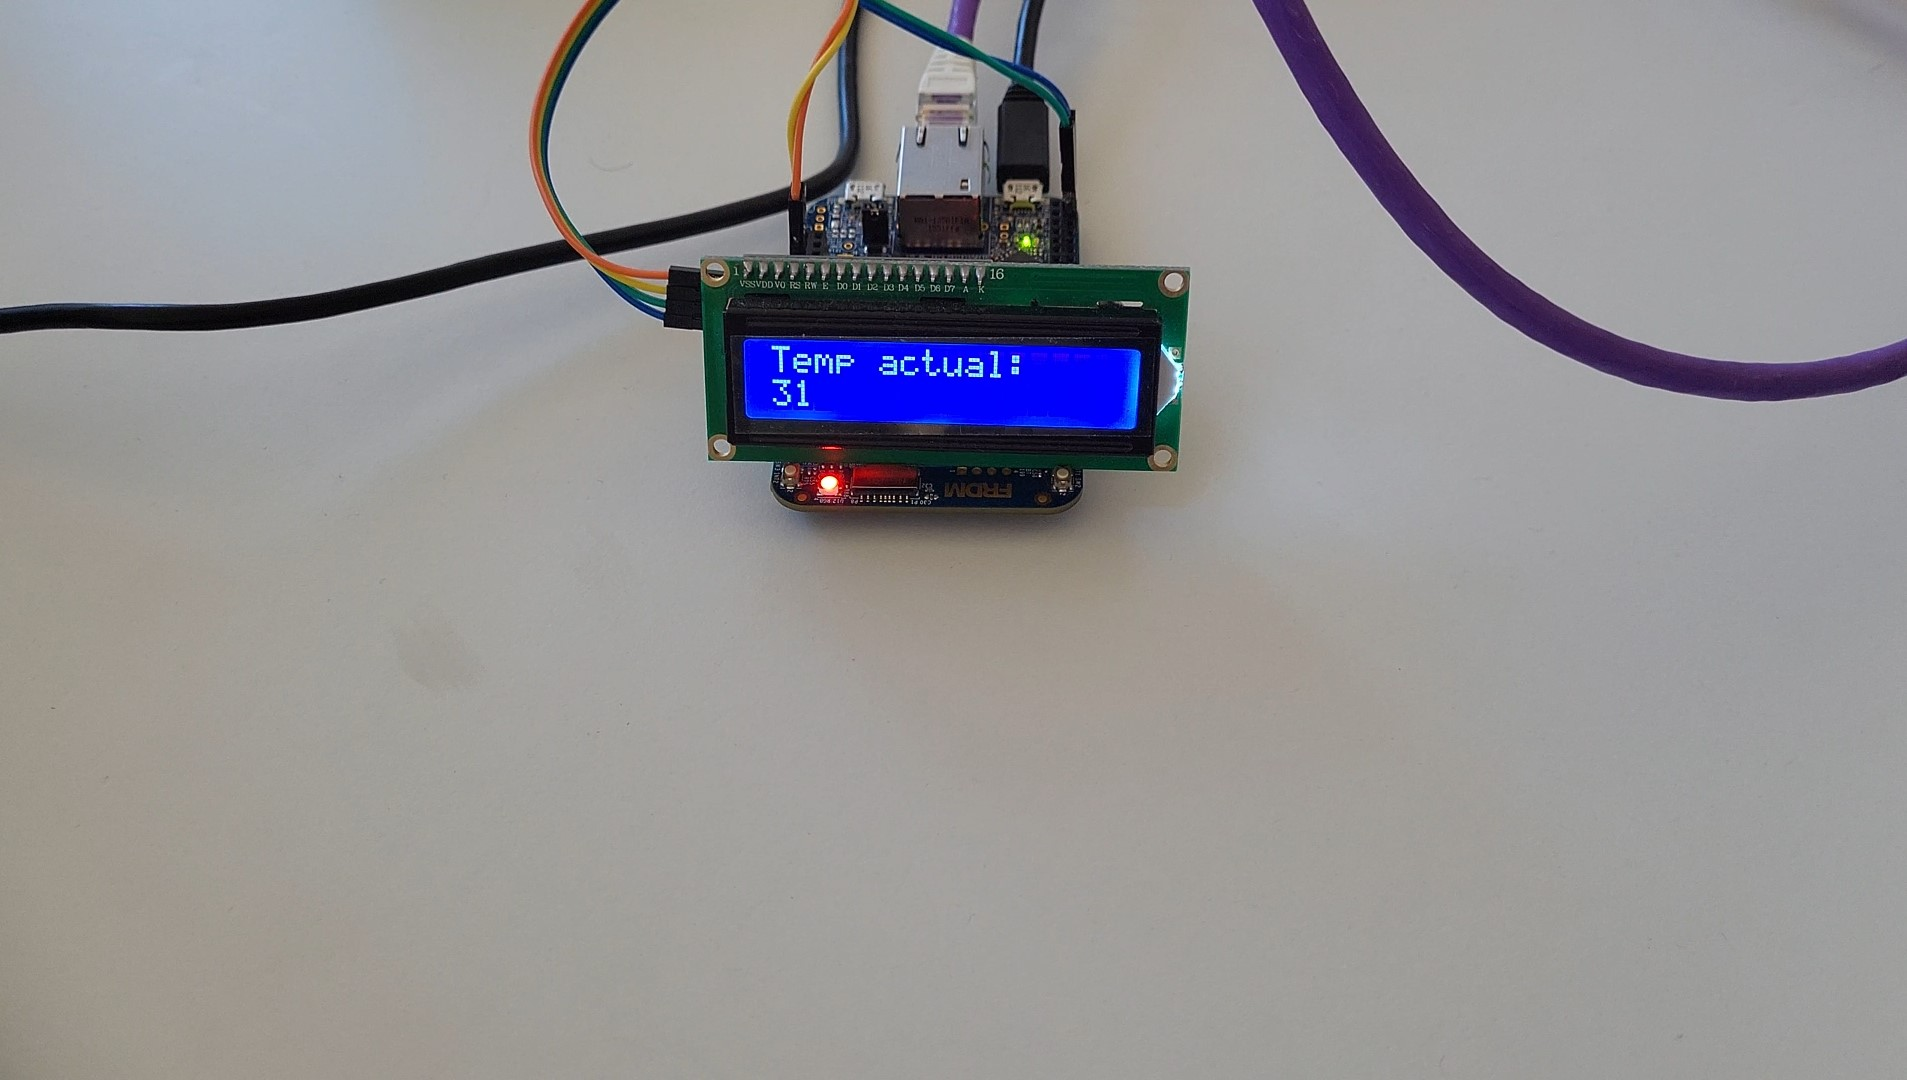
\includegraphics[width=0.4\textwidth]{CU31.png}}
  \subfloat[Temp: 34 grados]{
    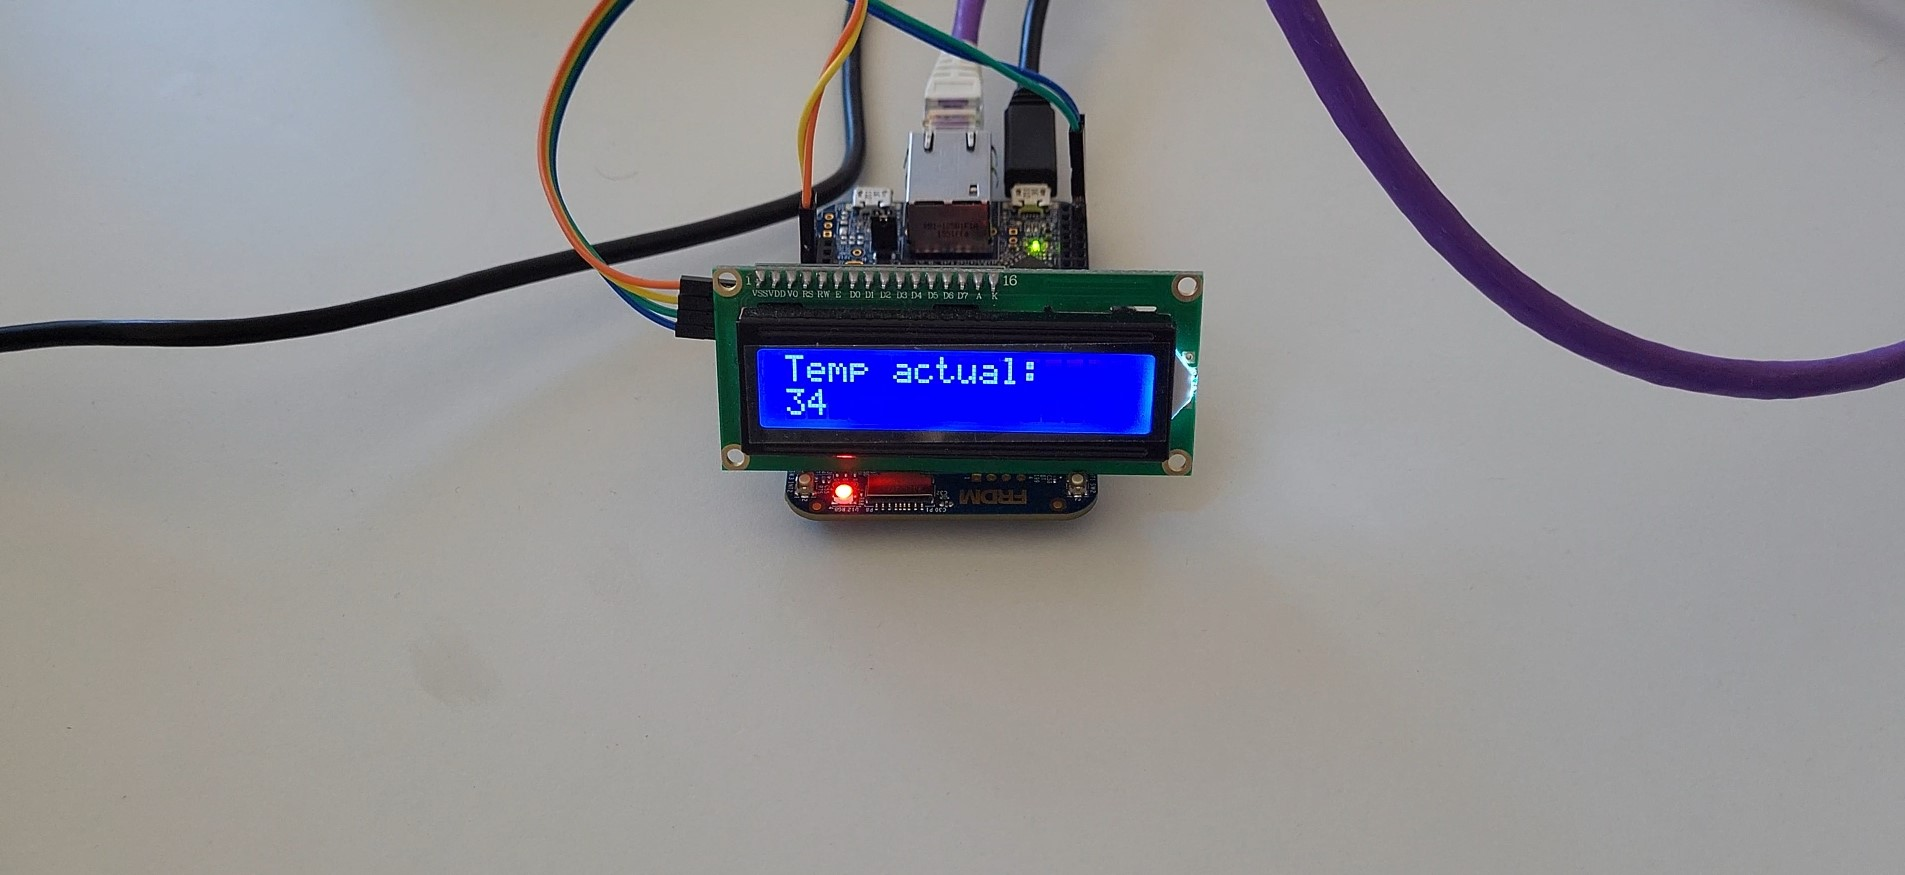
\includegraphics[width=0.475\textwidth]{CU34.png}}
 \caption{Caso de uso Kronospan.}
\end{figure}

\clearpage

En la Figura \ref{CPD} vemos como la placa maestro está introducida en el CPD para la captación de la temperatura.
%\imagen{CUCPD}{Placa `Maestro' en el CPD.} \label{CPD}
\begin{figure}[!h]
	\centering
	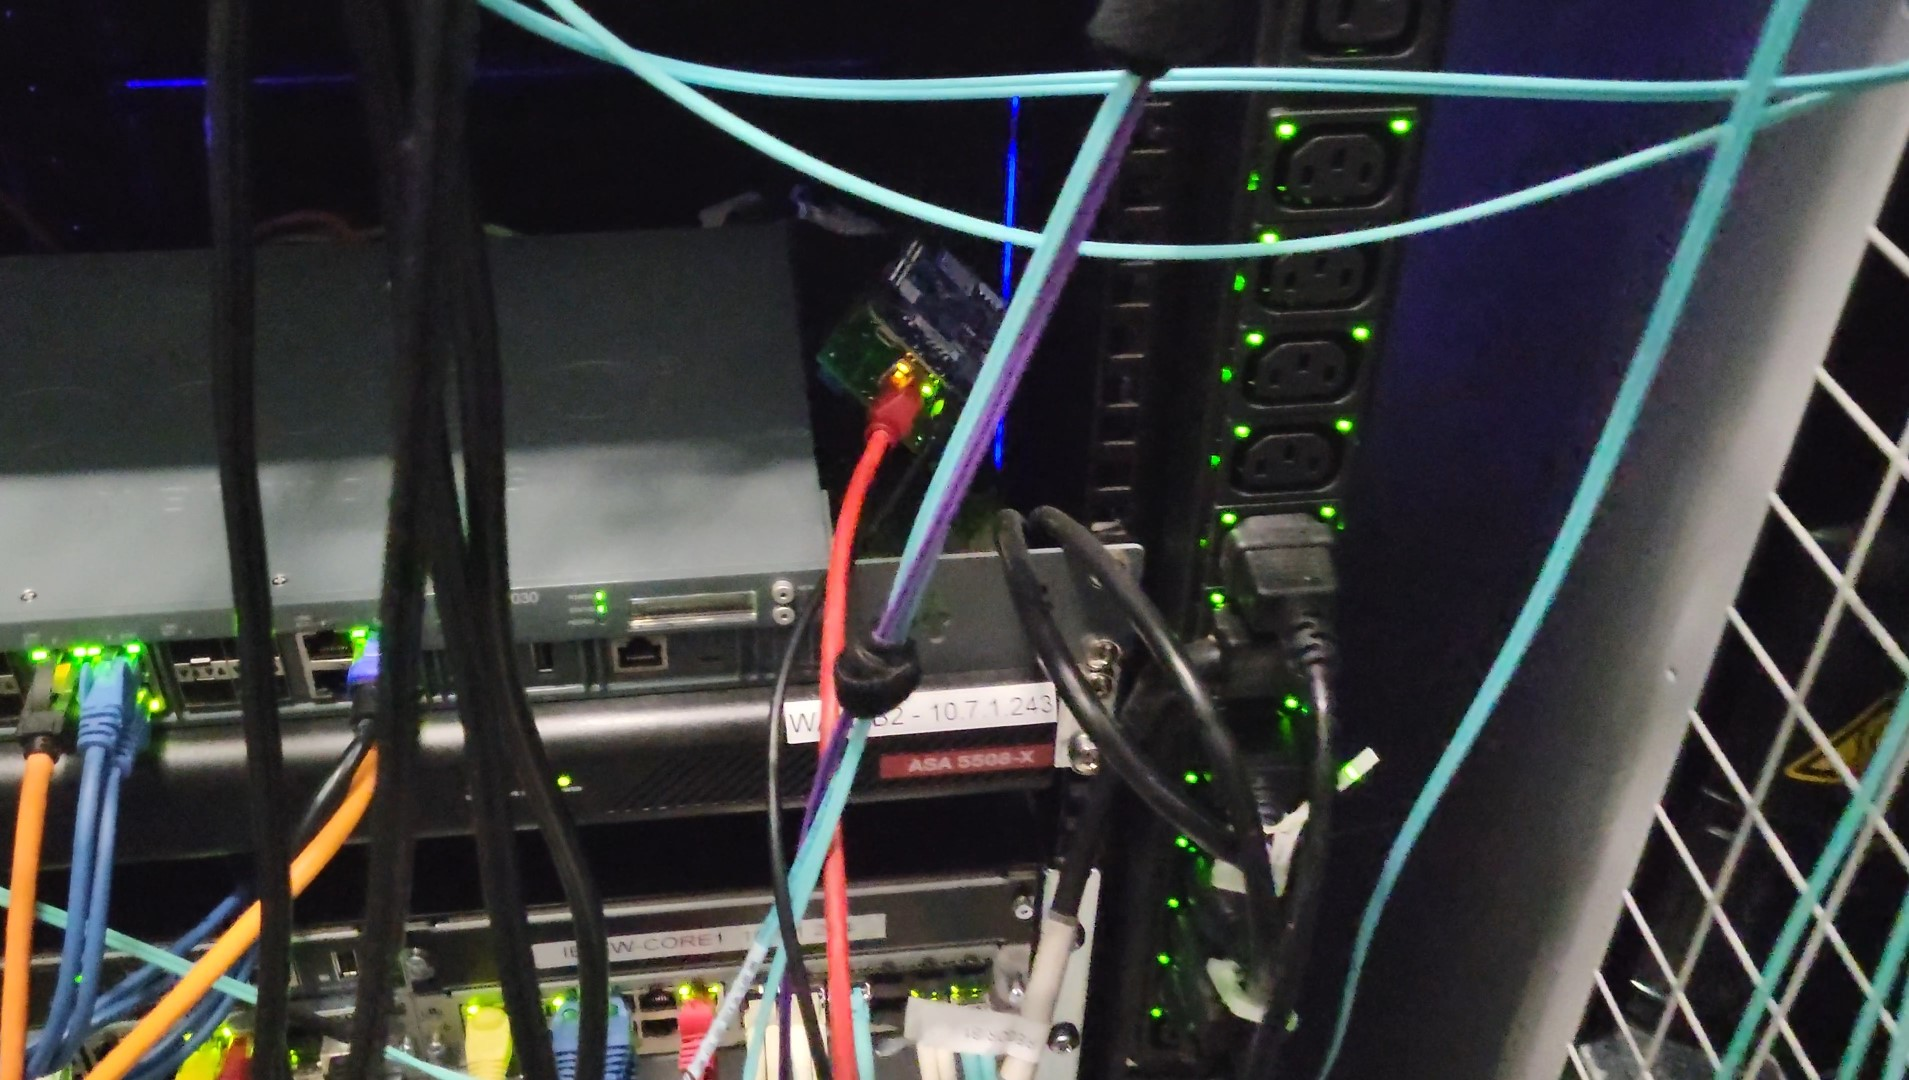
\includegraphics[width=0.9\textwidth]{CUCPD}
	\caption{Placa `Maestro' en el CPD.}\label{CPD}
\end{figure}

Estos han sido los hitos que más dificultades me han causado durante la realización del TFG.









